\documentclass[14pt,a4paper,report]{ncc}
\usepackage[a4paper, mag=1000, left=2.5cm, right=1cm, top=2cm, bottom=2cm, headsep=0.7cm, footskip=1cm]{geometry}
\usepackage[utf8]{inputenc}
\usepackage[english,russian]{babel}
\usepackage{indentfirst}
\usepackage[dvipsnames]{xcolor}
\definecolor{battleshipgrey}{rgb}{0.52,0.52,0.51}
\usepackage[colorlinks]{hyperref}
\usepackage{listings} 
\usepackage{caption}
\usepackage{amssymb}
\usepackage{tcolorbox}
\lstloadlanguages{[LaTeX]TeX,C++}
\DeclareCaptionFont{white}{\color{white}} 
\DeclareCaptionFormat{listing}{\colorbox{gray}{\parbox{\textwidth}{#1#2#3}}}
\captionsetup[lstlisting]{format=listing,labelfont=white,textfont=white}
\lstset{% Собственно настройки вида листинга
inputencoding=utf8, extendedchars=\true, keepspaces = true, % поддержка кириллицы и пробелов в комментариях
language=C++,            % выбор языка для подсветки 
numberstyle =\tiny
basicstyle=\small\sffamily, % размер и начертание шрифта для подсветки кода
keywordstyle =\color{RoyalPurple},
numbers=left,               % где поставить нумерацию строк (слева\справа)
numberstyle=\tiny,          % размер шрифта для номеров строк
stepnumber=1,               % размер шага между двумя номерами строк
numbersep=5pt,              % как далеко отстоят номера строк от подсвечиваемого кода
backgroundcolor=\color{white}, % цвет фона подсветки - используем \usepackage{color}
showspaces=false,           % показывать или нет пробелы специальными отступами
showstringspaces=false,     % показывать или нет пробелы в строках
showtabs=false,             % показывать или нет табуляцию в строках
frame=single,               % рисовать рамку вокруг кода
tabsize=2,                  % размер табуляции по умолчанию равен 2 пробелам
captionpos=t,               % позиция заголовка вверху [t] или внизу [b] 
breaklines=true,            % автоматически переносить строки (да\нет)
breakatwhitespace=false,    % переносить строки только если есть пробел
escapeinside={\%*}{*)}      % если нужно добавить комментарии в коде
}

\begin{document}
% Переоформление некоторых стандартных названий
%\renewcommand{\chaptername}{Курсовая работа}
\def\contentsname{Содержание}

\begin{titlepage}
\begin{center}
\vspace{5em}
\small Министерство образования и науки Российской Федерации

\small Федеральное государственное автономное образовательное учреждение высшего образования\\
\vspace{2em}
\normalsize \bf «Уральский федеральный университет

имени первого Президента России Б.\,Н.~Ельцина»

\bigskip
\vspace{1em}
\footnotesize \rm Физико-технологический институт

Кафедра теоретической физики и прикладной математики

\vspace{3em}
\large Пояснительная записка к курсовой работе по теме\\
\textsc{реализация многопотокового алгоритма численного решения классической спиновой модели методом глобальной оптимизации при помощи библиотеки MPI}\\
\end{center}
\vfill
\hfill

\begin{flushright}
\begin{minipage}{.5\textwidth}
Работа студента\\[1mm] 
группы ФтМ - 170403\\
Вяловой С.А.\\[5mm]

Преподаватель:\\[1mm] 
д.ф.-м.н., профессор\\
Мазуренко В.В.\\[5mm]

Консультант:\\[1mm] 
м.н.с.\\
Медведева Д. С.\\
\end{minipage}
\end{flushright}


\vfill
\begin{center}
Екатеринбург \\
2018
\end{center}
\end{titlepage}

\tableofcontents
%\renewcommand{\contentsname}{Содержание}
\newpage

\chapter*{Введение}
\addcontentsline{toc}{chapter}{Введение}
В настоящее время ряд задач, требующих для своего решения применения мощных вычислительных ресурсов, стремительно расширяется. Это связано с тем, что происходят фундаментальные изменения в самой организации научных исследований. Вследствие широкого внедрения вычислительной техники, значительно усилилось направление численного моделирования и численного эксперимента. Численное моделирование, заполняя промежуток между физическими экспериментами и аналитическими подходами, позволило изучать явления, которые являются либо слишком сложными для исследования аналитическими методами, либо слишком дорогостоящими или опасными для экспериментального изучения. При этом численный эксперимент позволил значительно удешевить процесс научного и технологического поиска. Стало возможным моделировать в реальном времени процессы интенсивных физико-химических и ядерных реакций, глобальные атмосферные процессы, процессы экономического и промышленного развития регионов и т.д. Очевидно, что решение таких масштабных задач требует значительных вычислительных ресурсов \cite{litlink0}. Это ставит перед нами задачу уменьшения времени, затрачиваемого на вычисления.
\

Вследствие вышесказанного, актуальной становится разработка программ, которые могут запускаться в параллельном режиме. Для этого могут быть использованы разные подходы, среди которых можно выделить интерфейс MPI (Message Passing Interface) -- библиотеку функций, обеспечивающую взаимодействие параллельных процессов с помощью механизма передачи сообщений \cite{litlink1}.
\

Ряд задач в теоретической физике требуют численного решения классических спиновых моделей. Проблема заключается заключается в поиске глобального минимума энергии таких систем. Поскольку зачастую есть необходимость решить такую задачу для большого числа однотипных спиновых систем, то, с точки зрения времени, затраченного на вычисления, разумно ее выполнять параллельно в несколько потоков.

\
Таким образом, целью данной работы является реализация многопотокового алгоритма численного решения классической спиновой модели методом глобальной оптимизации при помощи библиотеки функций MPI, а также оценка преимуществ проведения серии расчётов при помощи многопоточной программы относительно однопоточной программы. Для достижения поставленных целей были поставлены следующие задачи:
\begin{itemize}
\item Проанализировать имеющееся программное решение поставленной задачи;
\item разработать параллельную версию программы, пригодную для запуска на различных типах машин;
\item сравнить время выполнения данной задачи, выполняющейся в один поток и в несколько потоков.
\

Объектом данной курсовой работы является параллельное исполнение программы на CPU, предметом - классическая спиновая модель.
\end{itemize} 

\chapter*{Теоретическая часть}
\refstepcounter{chapter}
\addcontentsline{toc}{chapter}{1. Теоретическая часть}

\section{MPI (Message Passing Interface)}
\subsection{Терминология и обозначения}
Интерфейс MPI представляет собой набор утилит и библиотечных функций для языков C/C++ и FORTRAN, позволяющих создавать и запускать приложения, работающие на параллельных вычислительных установках \cite{Bogachev}.
MPI-программа -- это множество параллельных взаимодействующих процессов. Все процессы порождаются один раз, образуя параллельную часть программы. Каждый процесс работает в своем адресном пространстве, никаких общих переменных или данных в MPI нет. Основным способом взаимодействия между процессами является явная посылка сообщений. 
\

Для локализации взаимодействия параллельных процессов программы можно создавать группы процессов, предоставляя им отдельную среду для общения - коммуникатор. Состав образуемых групп произволен. Группы могут полностью совпадать, входить одна в другую, не пересекаться или пересекаться частично. Процессы могут взаимодействовать только внутри некоторого коммуникатора. а сообщения, отправленные в разных коммуникаторах, не пересекаются и не мешают друг другу. Коммуникаторы имеют в языке Фортран тип \textbf{INTEGER}. 
\

При старте программы всегда считается, что все порожденные процессы работают в рамках всеобъемлющего коммуникатора, имеющего предопределенное имя \textbf{MPI\_COMM\_WORLD}. Этот коммуникатор существует и всегда служит для взаимодействия всех запущенных процессов MPI-программы. Кроме него при старте программы имеется коммуникатор \textbf{MPI\_COMM\_SELF}, содержащий только текущий процесс, и коммуникатор \textbf{MPI\_COMM\_NULL}, не содержащий ни одного процесса. Все взаимодействия процессов протекают в рамках определённого коммуникатора, а сообщения, переданные в разных коммуникаторах, никак не мешают друг другу.
\

Каждый процесс MPI-программы имеет в каждой группе, в которую он входит, уникальный атрибут номер процесса, который является целым неотрицательным числом. С помощью этого атрибута происходит значительная часть взаимодействия процессов межлу собой. В одном и том же коммуникаторе все процессы имеют различные номера, но, поскольку процесс может одновременно входить в разные коммуникаторы, то его номер в одном коммуникаторе может отличаться от его номера в другом. Отсюда становятся понятными два основных атрибума процесса: коммуникатор и номер в коммуникаторе.

\
Посылка сообщений - основной способ общения процессов между собой. Сообщение - это набор данных некоторого типа. Каждое сообщение имеет несколько атрибутов, в частности, номер процесса-отправителя, номер процесса-получателя, идентификатор сообщения и другие. Одним из важных атрибутов сообщения является его идентификатор или тэг. По идентификатору процесс, принимающий сообщение, может различать два сообщения, пришедшие к нему от одного и того же процесса. Сам идентификатор сообщения является целым неотрицательным числом, лежащим в диапазоне от 0 до \textbf{MPI\_TAG\_UP}, и гарантируется, что \textbf{MPI\_TAG\_UP} не меньше 32767.
\footnote{Для описния использованных директив использован Антонов А.С. Учебное пособие "Параллельное программирование с использованием MPI".}
\subsection{Общие процедуры MPI}
Рассмотрим ряд процедур, необходимых в каждой содержательной параллельной программе.
\
\begin{itemize}
\item \textbf{MPI\_INIT(IERR)}
\

\textbf{INTEGER IERR}
\
\end{itemize}
Инициализация параллельной части программы. Все другие процедуры MPI могут быть вызваны только после вызова \textbf{MPI\_INIT}. Инициализация параллельной части для каждого приложения должна выполняться только один раз.
\
\begin{itemize}
\item \textbf{MPI\_FINALIZE(IERR)}
\

\textbf{INTEGER IERR}
\
\end{itemize}
Завершение параллельной части приложения. Все последующие обращения к любым процедурам MPI, в том числе  \textbf{MPI\_INIT(IERR)}, запрещены. К моменты вызова  \textbf{MPI\_FINALIZE(IERR)} каждым процессов программы все действия, требующие его участия в обмене сообщениями, должны быьть завершены
\begin{itemize}
\item \textbf{MPI\_COMM\_SIZE(COMM, SIZE, IERR)}
\

\textbf{INTEGER COMM, SIZE,  IERR}
\
\end{itemize}
В аргументе \textbf{SIZE} процедура возвращает число параллельных процессов в коммуникаторе  \textbf{COMM}. 

\
\subsection{Передача/прием сообщеий между отдельными процессами}
Практически все программы, написанные с использованием коммуникационной технологии MPI, должны содержать средства не только для порождения и завершения параллельных процессов, но и для взаимодействия запущенных процессов между собой. Такое взаимодействие и осуществляется в MPI посредством явной посылки сообщений.
\

Все процедуры передачи сообщений в MPI делятся на две группы. В одну группу входят процедура, которые предназначены для взаимодейсвия только двух процессов программы. Такие операции называются индивидуальными или операциями типа точка-точка. Процедуры другой группы предполагают, что в операцию должны быть вовлечены все процессоры некоторого коммуникатора. Такие операции называются коллективными.
\

Рассмотрим процедуры обмена сообщениями на примере операций типа точка-точка. В таких взаимодействиях участвуют два процесса, причём один процесс является отправителем сообщения, а другой - получателем. Процесс-отправитель должен вызвать одну из процедур передачи данных и явно указать номер в некотором коммуникаторе процесса-получателя, а процесс-получатель должен вызвать одну из процедур приема с указанием того же коммуникатора.

\ 
Все процедуры данной группы, в свою очередь, делятся на два класса: процедуры с блокировкой (с синхронизацией) и процедуры без блокировки (асинхронные). Процедуры обмена с блокировкой приостанавливают работу процесса до выполнения некоторого условия, а возврат из асинхронных процедур происходит немедленно после инициализации соответствующей коммуникационной операции.
\
\subsection{Передача /прием сообщеий с блокировкой}  
\begin{itemize}
\item\textbf{MPI\_SEND(BUF, COUNT, DATATYPE, DEST, MSGTAG,\\
 COMM, IERR)}
\

\textbf{<type> BUF(*)}
\

\textbf{INTEGER COUNT, DATATYPE, DEST, MSGTAG, COMM, IERR}
\
\end{itemize}
Блокирующая посылка массива \textbf{BUF} с идентификатором \textbf{MSGTAG}, состоящего из \textbf{COUNT} элементов типа \textbf{DATATYPE}, процессу с номером \textbf{DEST} в коммуникаторе \textbf{COMM}. Все элементы посылаемого сообщения должны быть расположены подряд в буфере \textbf{BUF}. Операция начинается независимо от того, быа ли инициализирована соответствующая процедура приема. Значение \textbf{COUNT} может быть нулем. Процессу разрешается передавать сообщение самому себе, однако это может привести к возникновению тупиковой ситуации.
\


Блокировка гарантирует корректность повторного использоваия всех параметров после возврата из процедуры. Это означает, что после возврата из \textbf{MPI\_SEND} можно использоват любые присутствующие в вызове данной процедуре переменные без опасения испортить передаваемое сообщение.
\begin{itemize}
\item\textbf{MPI\_RECV(BUF, COUNT, DATATYPE, DEST, MSGTAG,\\ COMM,
 STATUS, IERR)}
\

\textbf{<type> BUF(*)}
\

\textbf{INTEGER COUNT, DATATYPE, DEST, MSGTAG, COMM, IERR, STATUS(MPI\_STATUS\_SIZE)}
\
\end{itemize}
Блокирующий прием в буфер \textbf{BUF} не более \textbf{COUNT} элементов сообщения типа \textbf{DATATYPE} с идентификатором \textbf{MSGTAG} от процесса с номером \textbf{SOURCE} в коммуникаторе \textbf{COMM} с заполнением массива атрибутов приходящего сообщения \textbf{STATUS}. Если число принятых элементов меньше значения \textbf{COUNT}, то гарантируется что в буфере \textbf{BUF} изменятся только элементы, соответствующие элементов принятого сообщения. Если количество элементов в принимаемом сообщении больше значения \textbf{COUNT}, то возникает ошибка переполнения.

\subsection{Коллективные взаимодействия процессов}
В операциях коллективного взаимодействия процессов участвуют все процессы коммуникатора. Соответствующая процедура может быть вызвана каждым процессом со своим набором параметров. Возврат из процедуры коллективного взаимодействия может произойти в тот момент, когда участие процесса в данной операции уже закончено. Как и для блокирующих процедур, возврат означает то, что разрешен свободный доступ к буферу приема или посылки.
\

В коллективных операциях не используются идентификаторы сообщений (теги). Таким образом, коллективные операции строго упорядочены согласно их появлению в тексте программы.
\begin{itemize}


\item\textbf{MPI\_BARRIER(COMM, IERR)}
\

\textbf{INTEGER COMM, IERR}
\
\end{itemize}
Процедура используется для барьерной синхронизации процессов. Работа процессов блокируется до тех пор, пока все оставшиеся процессы коммуникатора \textbf{COMM} не выполнят эту процедуру. Только после того, как последний процесс коммуникатора выполнит данную процедуру, все процессы будут разблокированы и продолжат выполнение дальше. Данная процедура является коллективной. Все процессы должны вызвать \textbf{MPI\_BARRIER}, хотя реально исполненные вызовы различными процессами коммуникатора могут быть расположены в разных местах программы.
\begin{itemize}
\item\textbf{MPI\_BCAST(BUF, COUNT, DATATYPE, ROOT, COMM, IERR)}

\textbf{INTEGER COUNT, DATATYPE, ROOT, COMM, IERR}
\end{itemize}
Рассылка \textbf{COUNT} элементов данных типа \textbf{DATATYPE} из массива \textbf{BUF} от процесса \textbf{ROOT} всем процессам данного коммуникатора \textbf{COMM}, включая сам рассылающий процесс. При возврате из процедуры содержимое буфера \textbf{BUF} процесса \textbf{ROOT} будет скопировано в локальный буфер каждого процесса коммуникатора \textbf{COMM}. Значения параметров \textbf{COUNT}, \textbf{DATATYPE},  \textbf{ROOT} и \textbf{COMM} должны быть одинаковыми у всех процессов.
\


\chapter*{Практическая часть}
\refstepcounter{chapter}
\addcontentsline{toc}{chapter}{2. Практическая часть}
%\addcontentsline{toc}{chapter}{Практическая часть}
\section{Параметры системы}
Сборка и запуск программы велись в коммандной оболочке Bash при помощи утилит mpifort и mpirun из пакета mpich.
\footnote{MPICH is a high performance and widely portable implementation of the Message Passing Interface (MPI) standard.}
В качестве платформ для тестирования были использованы машины со следующими параметрами: 
\begin{itemize}


\item операционная система Gentoo GNU/Linux. Процессор Intel(R) Core(TM) i3-3110M 2.40GHz, ОЗУ 6,00 Гб.
\item операционная система Debian GNU/Linux. Процессор Intel(R) Core(TM) i7-3770 3.40GHz, ОЗУ 8,00 Гб.
\end{itemize}
\section{Параметры запуска и блок-схема программы}

Рассматриваемый программный код решает задачу поиска глобального минимума энергии как функции многих переменных для заданного количества однотипных спиновых систем. Начальные параметры спиновых систем задаются при помощи трёх конфигурационных файлов - Basic, Exchange и Frozen. Начальные направления спинов задаются хаотически для каждой спиновой системе в программе.
\

Входные файлы содержат значения следующих входных параметров:
\begin{itemize}
\item $N\_Spins$ - число спинов в системе;
\item $H\_mag$ - величина магнитного поля;
\item $N\_Steps$ - число конфигураций, для которых будет посчитан глобальный минимум энергии;
\item $num$ - номер спина и соответствующий ему модуль обменного коэффициента S\_Value;
\item $N\_Couples$ - число взаимодействующих спиновых пар;
\item $Exchange$ - коэффициент обменного взаимодействия для каждой пары;
\item $N\_Frozen$ - число замороженных спинов.
\end{itemize}
\ 
На выходе программы для каждого уникального состояния генерируются файлы, содержащие следующую информацию:
\

\begin{itemize}
\item Энергия полученного состояния;
\item номера спинов; 
\item продольный и поперечные углы, соответсвующие каждому спину;
\item магнитный момент каждого спина;
\item суммарный магнитный момент системы.
\end{itemize}
\

Блок-схема программы представлена на рисунке \ref{ris:image1}.
Поскольку рассматриваемая программа производит расчёт $N\_Steps$ конфигураций системы, то среди полученных конфигураций встречаются такие, минимальные энергии которых одинаковы. Записывать в выходные файлы повторяющиеся конфигурации не имеет смысла, поэтому в программе реализован анализ состояний при помощи соответствующей подпрограммы $State\_Analysis$. Блок-схема данной подпрограммы представлена на рисунке \ref{ris:image2}.

\begin{figure}[p]
\center{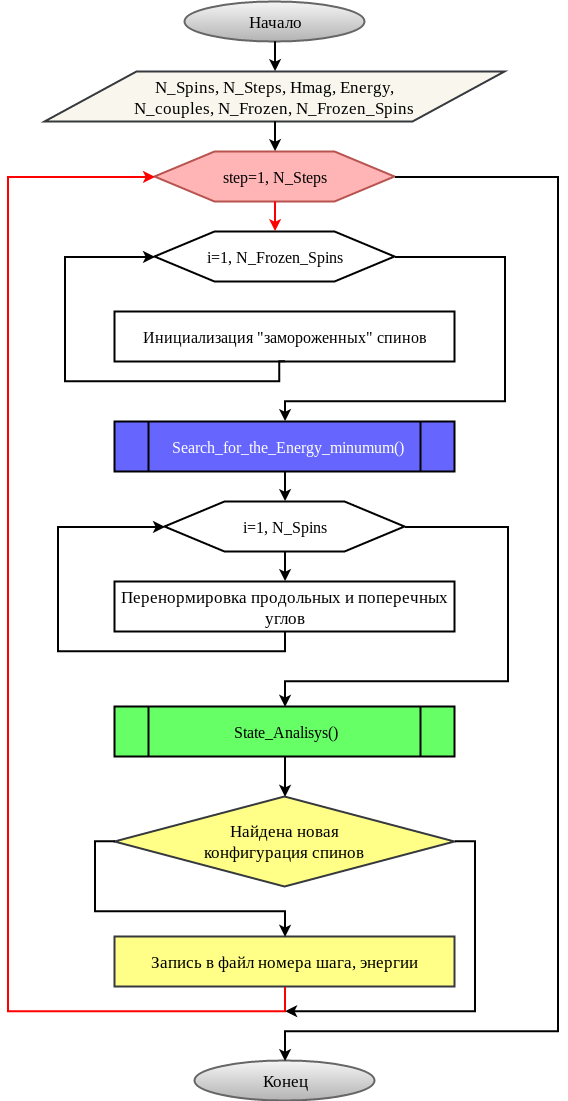
\includegraphics[width=0.7\linewidth]{program_NoMPI.png}}
\caption{Блок-схема программы.}
\label{ris:image1}
\end{figure}
\

\begin{figure}[p]
\center{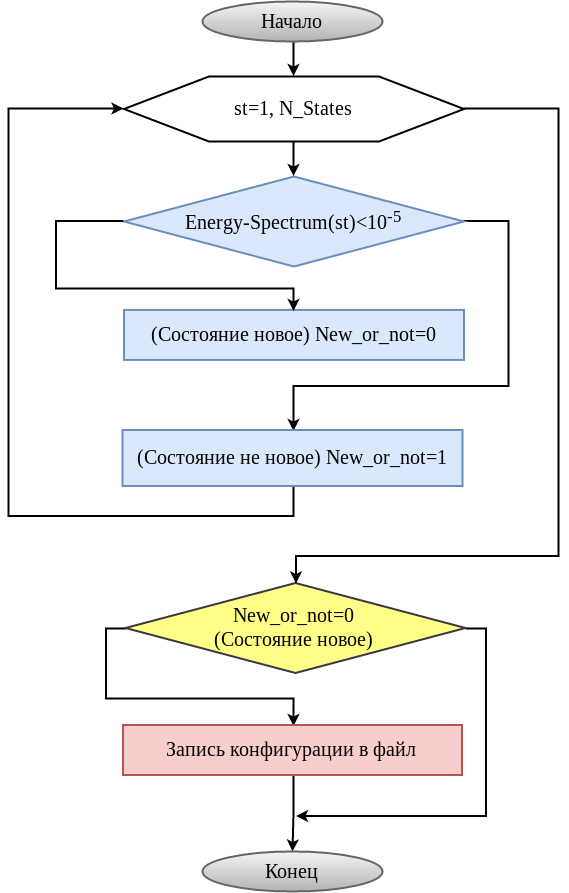
\includegraphics[width=0.7\linewidth]{subroutine_NoMPI.png}}
\caption{Блок-схема подпрограммы State\_Analysis.}
\label{ris:image2}
\end{figure}
\

\newpage
\section{Разработка паралелльной версии программы. Технология MPI}

Расчёт параметров основного состояния спиновой модели(энергии, продольного и поперечного углов спинов), реализованный в рассматриваемой программе, происходит в цикле, и параметры, необходимые для расчёта основного состояния, не пересекаются. Поэтому разумно блоки программ, реализующих расчёт данных величин, выполнять на разных процессорах. 
\


MPI позволяет решить задачу поиска глобального минимума энергии как функции многих переменных распределить на $N$ потоков, выполняющихся параллельно. Для этого основной цикл программы, в которой $N\_Steps$ раз вычисляется глобальный минимум энергии системы, начальное состояние которой задаётся произвольно, можно разбить на $N$ частей так, чтобы в каждом потоке считались $\frac{M}{N}$ конфигураций, соответствующих глобальному минимуму энергии системы.
\

Для этого необходимо разбить параметр $N\_Steps$ на $N$ частей. Тогда конечной точкой $step\_end$ для каждого потока c идентификатором $myid$ будет $step\_end = (myid+1)\cdot h$, где $h=\frac{N\_Steps}{N}$, а стартовой точкой $step\_begin$ для каждого потока будет число $step\_begin=step\_end - h +1$
\

Блок-схема параллельной версии программы представлена на рисунке \ref{ris:image4}.

Поскольку не все $N\_Steps$ конфигураций, соответствующих минимуму энергии системы, являются оригинальными, и многие полученные наборы состояний спинов повторяются, то в программе происходит отбор состояний, энергии которых отличаются, и лишь оригинальные состояния записываются в спектр. Этот блок программы также можно выполнять параллельно. Для этого назначим поток, идентификатор которого равен 0, главным потоком ($master$). После части кода, в которой выполняется поиск глобального минимума конфигурации, запускается процедура \textbf{MPI\_BARRIER}. Ее задача - блокировка выполнения дальнейших задач до момента вычисления минимума энергии на каждом из потоков.  В ходе отбора и записи этих состояний с остальных потоков на master значение минимума энергии будет последовательно передаваться процедурой \textbf{MPI\_SEND}. Главный поток, в свою очередь, процедурой \textbf{MPI\_RECV} будет принимать в переменную Energy\_current значение полученной с других потоков энергии, иначе в эту переменную записывается значение энергии, полученное на потоке с номером $master$. 
\

Чтобы потокам, идентификатор которых не соответствует потоку $master$, принять решение о записи в спектр нового состояния, им необходимо инициировать получение значения переменной $New\_or\_not$. Для этого каждый ненулевой поток после отправления на $master$ значения энергии инициируют получение значения переменной $New\_or\_not$ от потока $master$ процедурой \textbf{MPI\_RECV}. Поток с идентификатором master при этом должен отправить значение переменной $New\_or\_not$ процедурой \textbf{MPI\_SEND}. 
\

Таким образом происходит обмен сообщениями между потоками, которые на момент вызова \textbf{MPI\_BARRIER} хранят конфигурацию спинов, соответствующую минимуму энергии, а также само значение минимума энергии системы. Выполнение данной программы в несколько потоков уменьшает время выполнения программы за счёт того, что вычисление энергий и конфигураций происходит в $N$ потоков, а решение о записи конфигураций и энергий принимается только на одном потоке $master$ за счёт отправления ему лишь значения энергии с других потоков. Запись файлы спектра состояний и конфигураций, в свою очередь, снова происходит в $N$ потоков.
Блок-схема параллельной версии подпрограммы $State\_Analysis$ представлена на рисунках \ref{ris:image5} и \ref{ris:image6}.  Программный код параллельной версии программы доступен по ссылке \href{http://www.tug.org/}%
{\TeX\ User Group}.




\begin{figure}[p]
\center{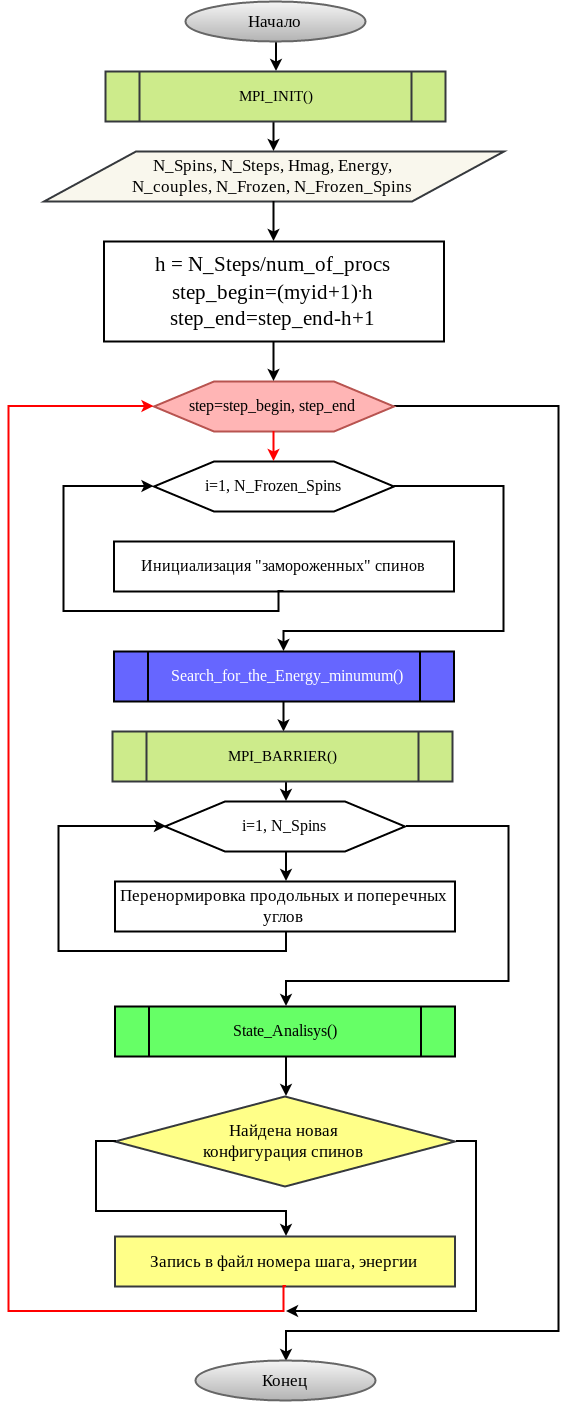
\includegraphics[width=0.5\linewidth]{program_MPI.png}}
\caption{Блок-схема параллельной версии программы .}
\label{ris:image4}
\end{figure}
\

\begin{figure}[p]
\center{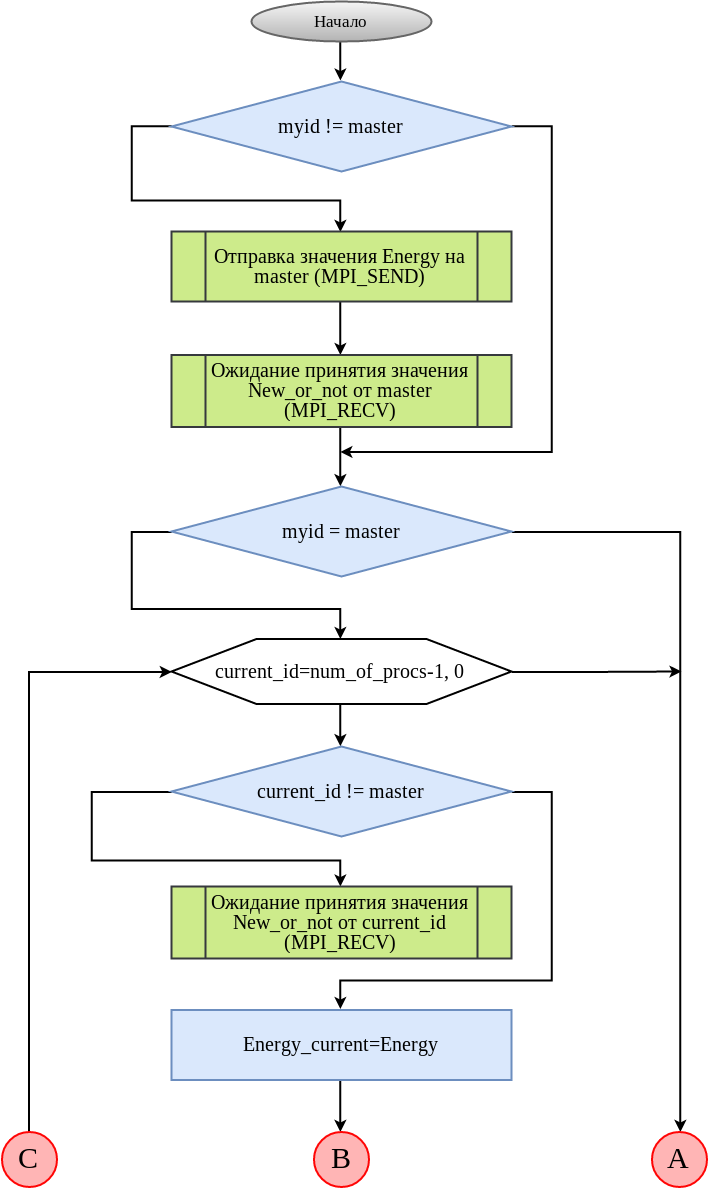
\includegraphics[width=0.7\linewidth]{subroutine_MPI_1.png}}
\caption{Блок-схема параллельной версии подпрограммы State\_Analysis (начало).}
\label{ris:image5}
\end{figure}
\

\begin{figure}[p]
\center{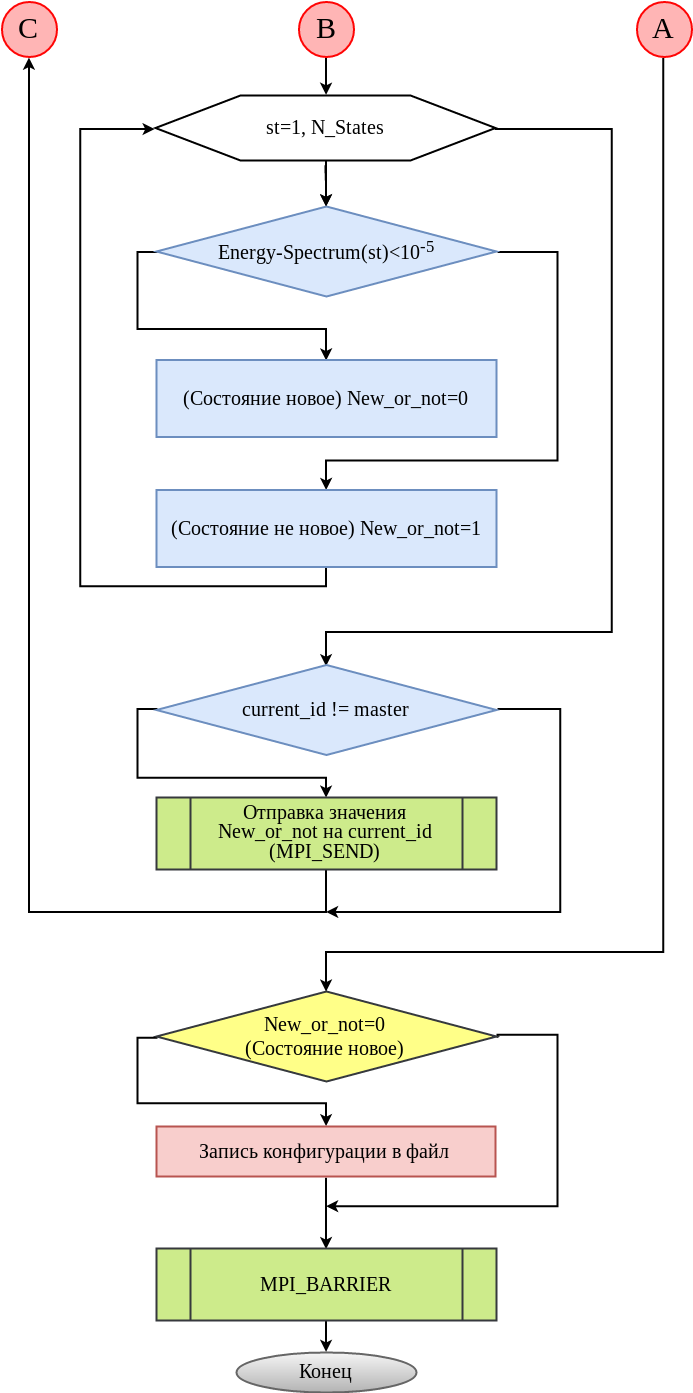
\includegraphics[width=0.7\linewidth]{subroutine_MPI_2.png}}
\caption{Блок-схема параллельной версии подпрограммы State\_Analysis (конец).}
\label{ris:image6}
\end{figure}
\

\newpage
\chapter*{Результаты}
\refstepcounter{chapter}
Разработанная параллельная версия программы запускалась при параметрах, представленных в таблице \ref{table_initial}, на двух машинах с одинаковым программным обеспечением, но на различных аппаратных платформах. 
\

Для начала сравним среднее время выполнения программы в зависимости от числа конфигураций $N\_Steps$, обсчитываемых программой, для Intel(R) Core(TM) i3-3110M 2.40GHz.
\

\
\begin{table}[h!]
\begin{center}
\caption{Входные данные, используемые для сравнения времени выполнения программы.}
\begin{tabular}{cccc}
Параметр & Значение \\
$N\_Spins$   & 20 \\
$N\_Couples$ & 27 \\
$H\_mag$ & 0.1 \\
$N\_Frozen$ & 1\\
 \end{tabular}
\label{table_initial}
\end{center}
\end{table}
\


График зависимости среднего времени выполнения программы для различных значений числа обсчитываемых конфигураций представлен на рисунке \ref{ris:image7}. Усреднение проводилось по пяти измерениям. Линия синего цвета соответствует среднему времени выполнения программы в четыре потока, линия красного цвета - среднему времени выполнения программы в два потока, и линия зеленого цвета соответствует времени выполнения программы в один поток. 
\

\begin{figure}[h!]
\center{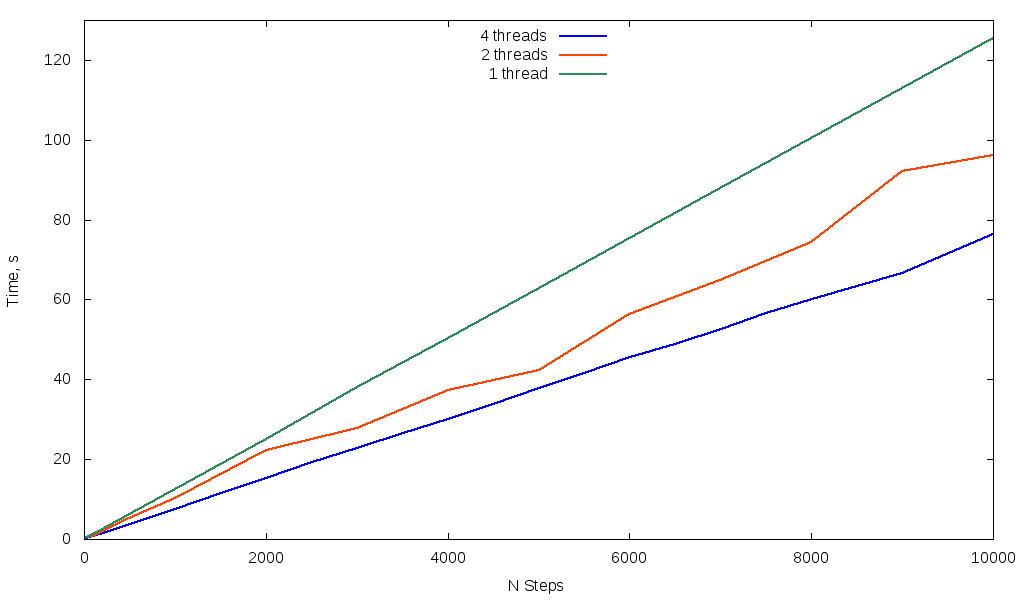
\includegraphics[width=0.65\linewidth]{program/time.png}}
\caption{График зависимости среднего времени выполнения программы для различных значений $N\_Steps$ на платформе Intel(R) Core(TM) i3-3110M 2.40GHz.
Синим цветом обозначено время выполнения программы на 4-х потоках; красным - на 2-х потоках; зеленым - на 1-м потоке.}
\label{ris:image7}
\end{figure}
\

Полученный график зависимости \ref{ris:image7} демонстрирует, что время выполнения параллельной версии программы в 4 потока в 1,64 раза меньше, нежели время выполнение однопоточной версии программы; программа, выполняемая в 2 потока, показала выигрыш по времени в 1,31 раз относительно однопоточной версии программы, что, однозначно, доказывает разумность выполнение такого типа задач в несколько потоков.
\

\begin{figure}[h!]
\center{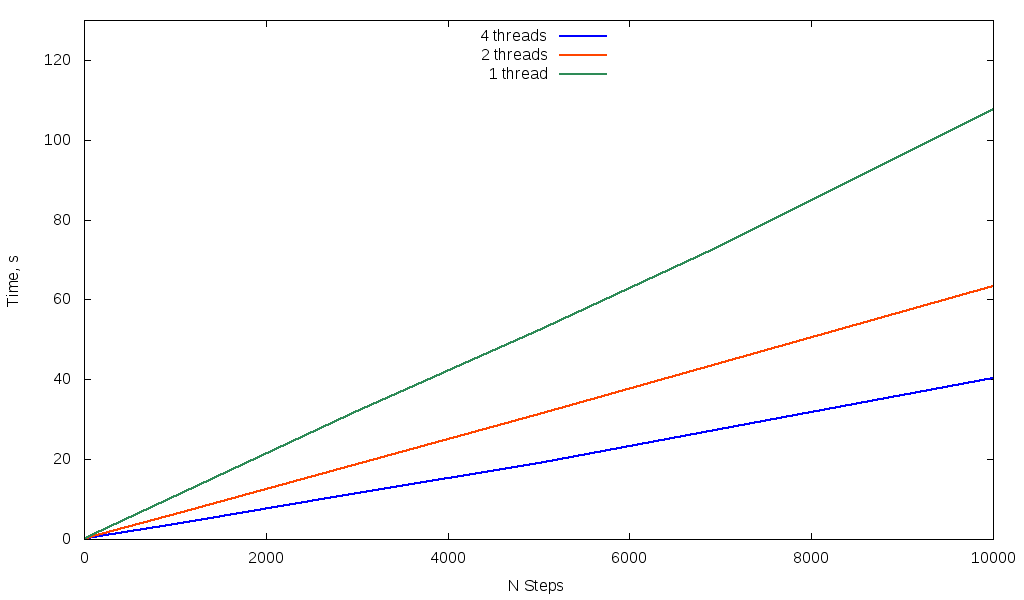
\includegraphics[width=0.65\linewidth]{program/time_job.png}}
\caption{График зависимости среднего времени выполнения программы для различных значений $N\_Steps$ на платформе Intel(R) Core(TM) i7-3770 3.40GHz.
Синим цветом обозначено время выполнения программы на 4-х потоках; красным - на 2-х потоках; зеленым - на 1-м потоке.}
\label{ris:image8}
\end{figure}
Рассмотрим теперь время выполнения программы для второй машины с процессором Intel(R) Core(TM) i7-3770 3.40GHz. График зависимости времени выполнения программы от значения $N\_Steps$ представлен на рисунке \ref{ris:image8}. Как и на графике \ref{ris:image7}, время выполнения программы в большее, чем один, число потоков приводит к большему выигрышу по времени относительно однопоточной программы. В данном случае время сократилось в 2,67 раз. Как и ожидалось, вычисления, производимые на более мощном процессоре, привели к уменьшению времени, затрачиваемого на выполнение программы в 4 потока. Здесь относительно менее мощного процессора выигрыш по времени составил 30\%. 
\

Таким образом, можно сделать однозначный вывод, что выполнение задач, подобных рассматриваемой, где имеет место большое количество независимых однотипных вычислений, разумно в несколько потоков. В данном случае имеет место прирост производительности, в среднем, в 2 раза. Также, для ускорения вычислений, для выполнения программ подобного рода разумным выбором будет более мощная аппаратная платформа. 
\chapter*{Заключение}
\addcontentsline{toc}{chapter}{Заключение}
В ходе данной работы была разработана параллельная версия программы, которая осуществляет численное решение классической спиновой модели методом глобальной оптимизации при помощи интерфейса MPI. Были оценены преимущества во времени выполнения для данной программы, которая тестировалась запусками в два и четыре потока, относительно однопоточной версии программы; также было проведено сравнение полученных результатов на двух различных машинах с одинаковой программной платформой, аппаратные платформы которых различаются по мощности.
\

В ходе тестирования был получен прирост производительности по времени многопоточной версии программы относительно однопоточной в 1,6 раз для более слабой аппаратной платформы и в 2,67 раз для более мощной аппаратной платформы. 

\
Исходя из результатов, был сделан вывод, что математические расчёты физических систем разумно выполнять в несколько потоков. Для разработки многопоточных программ MPI подтвердил свою эффективность. Более того, для большего прироста производительности эффективно использовать, одновременно с многопоточностью, более мощную аппаратную платформу.
 
% даём указание на включение данного место в оглавление как секции (\section)
%\addcontentsline{toc}{chapter}{Список использованных источников} 
 
\renewcommand{\bibname}{Список использованных источников}
\begin{thebibliography}{}
	\bibitem{Heisenberg}Вонсовский С. В., Магнетизм. Магнитные свойства диа-, пара-, ферро-, антиферро-, и ферримагнетиков. - М.: Изд-во ''Наука'' , 1971. - 1032 с.
   \bibitem{litlink0}Гэри М., Джонсон Д., Вычислительные машины и труднорешаемые задачи. - М.: Мир, 1982. - 416 с.   
   \bibitem{litlink1} Антонов А. С., Параллельное программирование с использованием технологии MPI:
Учебное пособие - М.: Изд-во МГУ, 2004. - 71 с
    \bibitem{litlink2} Корнеев В. Д., Параллельное программирование в MPI: Учебное пособие - М.: Изд-во ИВМиМГ, 2002. - 215 с.
    \bibitem{Bogachev} Богачёв К. Ю., Основы параллельного программирования: Учебное пособие - М.: Изд-во БИНОМ, 2015. - 345 с. 
     
\end{thebibliography}
\end{document}